\newpage
\hypertarget{allCards vis}{}
\subsection{AllOtherPartitionsRule}
\genHeader

Remember that you can start the majority of new rules in two different ways! You can either return to the TGG's \texttt{Rules} diagram and use the toolbox
there, or knowing that you need \texttt{box} and \texttt{partition0} for the context of the transformation, you can \emph{derive} this rule from 
\texttt{BoxToDictionaryRule}.

\begin{itemize}

\item[$\blacktriangleright$] Once you've initialized the \texttt{AllOtherPartitionsRule} diagram, build the rule until it matches
Fig.~\ref{fig:ea_AllOtherPartitionsRuleComplete}.

\begin{figure}[htbp]
\begin{center}
  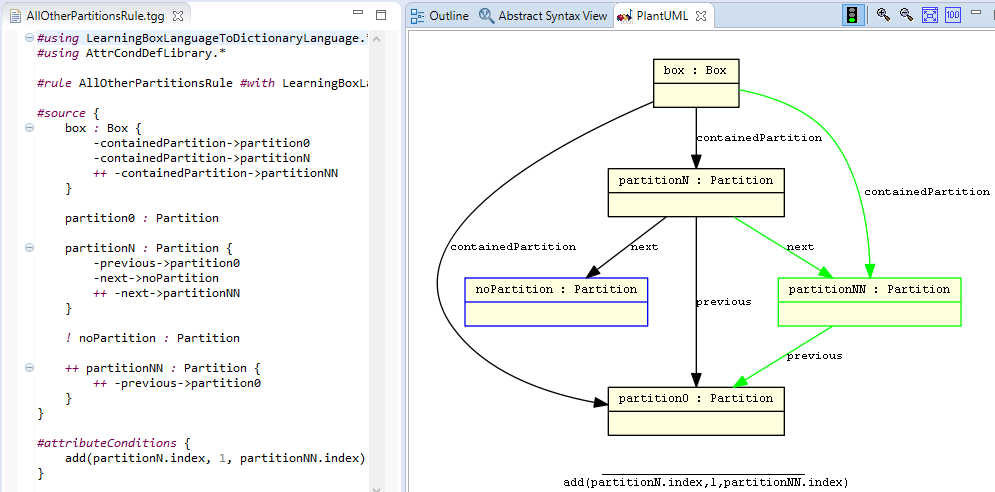
\includegraphics[width=0.7\textwidth]{ea_AllOtherPartitionsRule}
  \caption{The completed \texttt{AllOtherPartitionsRule}}
  \label{fig:ea_AllOtherPartitionsRuleComplete}
\end{center}
\end{figure}

\item[$\blacktriangleright$] As you can see, this rule doesn't assume to know the final \texttt{partition} in the transformation. It matches some
\texttt{n}th partition with an \texttt{index} 2 or more, then connects a new \texttt{n+1}th partition to \texttt{n} and \texttt{partition0}. 

\item[$\blacktriangleright$] Save, validate, export, and refresh your Eclipse package explorer to generate code for this rule. Run the TGG again -- it works!
The transformation is now able to handle the troublesome \texttt{next} dangling edge from the third partition.

\item[$\blacktriangleright$] Feel free to go ahead and add as many \texttt{partition}s and \texttt{card}s as you like to your model instance.
Your TGG is now
also able to handle a \texttt{box} with any number of \texttt{partition}s beautifully. 

\end{itemize}
